\chapter{Evaluation}\label{ch:evaluation}

For our experimental evaluation we split a monolithic dataflow computation into a
modular set of queries. The modular queries share their results in a topic,
allowing subscribers to further process the data. Because queries
can be dynamically added to the system, there is no need to interrupt the
running computation if additional analysis stages have to be added.

This increased flexibility comes however at a cost. As data has to be published
in topics in order to be accessed by consuming queries, we expect there to be
some overhead in both memory consumption and processing latency. The goal
of this chapter is to measure and analyze the overhead of query composition
on a realistic workload.

\paragraph{Experimental setup}

All experiments in this chapter are executed on a dual-socket Intel Xeon E5-2650
machine (2.0GHz, 8 cores per socket, 2 threads per core) with 64 GB RAM. All components and
queries in our system are compiled with a Rust 1.14 nightly build (2016-10-20)
and executed on Debian 7.8. The input data is read from a SAN storage attached
via iSCSI on a private 10 Gbit Ethernet network.

\section{Query composition for sessionization}

The dataflow computation in this experiment is based on \emph{sessionization},
i.e. the reconstruction of user sessions from a trace of log events.

\subsection{Computation \& workload}

The workload in this experiment is an hour-long trace of log events, collected in
a large datacenter owned by a travel company. The messages in our trace were
accumulated concurrently by 42 log servers, which received their log events from
1263 different streams. Events are originating from a distributed middleware which acts
as a message broker. It records metadata about the received messages, such as
timestamp, session identifer, and transaction identifer, and forwards them to
the log sever.

The computation we use on this workload is called \emph{sessionization}. Sessionization
is the reconstruction of user sessions, i.e. grouping and then processing all
messages belonging to the same session. For this purpose, the computation wait for
the arrival of late messages before it can consider the session closed. In
our experiment we use a fixed inactivity limit of 5 seconds, and re-order messages
within an event time window of 10 seconds. This is enough to incooperate more
than 99.99\% of all messages. 

While sessionization has been designed for real-time processing on a live
stream of events, we will load the workload trace from disk for our experiments.
This not only simplifies the experimental design and ensures reproducibility,
it also allows us to explore the behavior of the system if there are only a
few worker threads.

\subsection{Dataflow graph}

Input is read by from disk and fed into the dataflow graph in parallel, each worker
is responsible for a partition of the log servers. The read messages are sent
into the sessionization stage, where all messages belonging to the same session
are grouped together.

After the sessionization, the computation performs a set of statistics on the
reconstructed sessions. The stages are described below, the resulting dataflow
graph is shown in Figure~\ref{fig:monolith}

Messages are shuffeled according to their session identifier for the
sessionization stage, and are processed in parallel until statistics are
collected for the output, which is emitted at a single worker. 

\begin{description}
\item [Input] Parses the input files and feeds them into the sessionization stage.
\item [Sessionization] Distributes and then groups messages according to their session identifier.
Emits groups of messages belonging to the same session after a period of inactivity.
\item [Messages per Session] Simply counts and emits the number of messages belonging to a session.
\item [Duration of Session] Calculates the timespan between the first and last message of a session.
\item [Parse Transaction Trees] Parses the transaction identifiers for tree extraction.
\item [Transaction Tree Depth] Calculates the depth of the transaction trees.
\item [Top k Transaction Tree Signatures] Calculates signatures for the transaction trees and
reports the ten top most common tree signatures.
\item [Top k Communication Pairs] Infers the ten most common pairs of services who are
communicating with each other.
\item [Output] Collects emitted data in a histogram.
\end{description}

\subsubsection{Splitting up the dataflow graph}

For this evaluation we split up the computation such that each stage represents
its own sub-query. In order to achieve this, we introduce two topics: The topic
\emph{sessionize} contains the result of the sessionization stage, i.e. 
the groups of messages belonging to a session. The second topic, named
\emph{transactions}, is introduced for the transaction-oriented statistics.
It emits a stream containing all the transactions per session. The resulting
modular dataflow graph is shown in Figure~\ref{fig:split}, it consists of
seven queries, each one running in its own operating system process.

\begin{figure}[p]
  \centering
    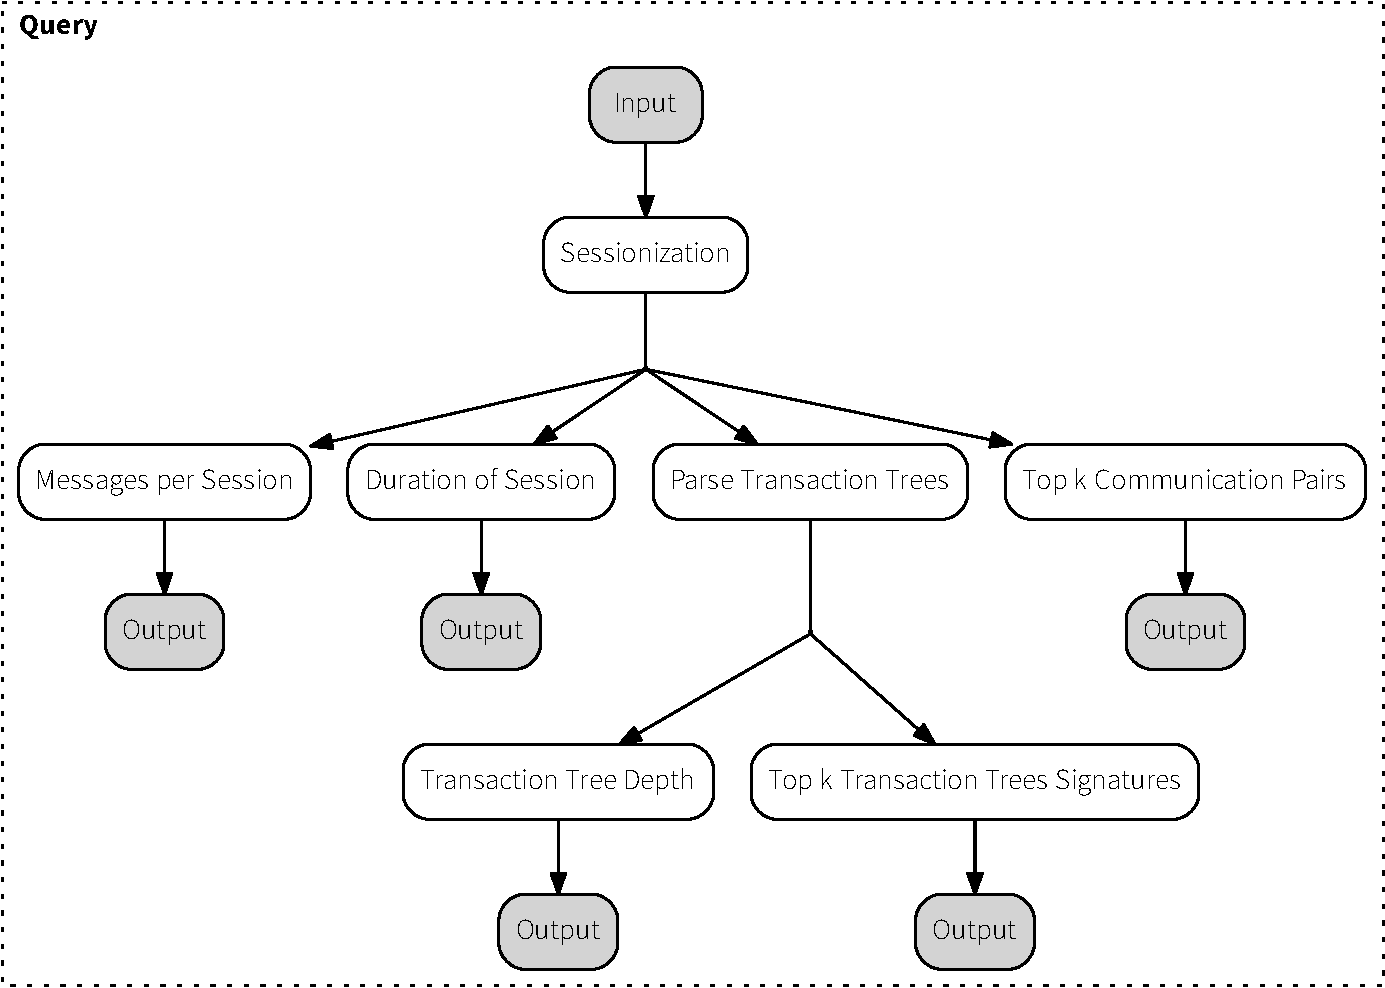
\includegraphics[width=1\textwidth]{figures/sessionize_dataflow-crop}
  \caption[Dataflow graph for monolithic sessionization]{The dataflow graph
  for the original, monolithic sessionization query.}
  \label{fig:monolith}
\end{figure}

\begin{figure}[p]
  \centering
    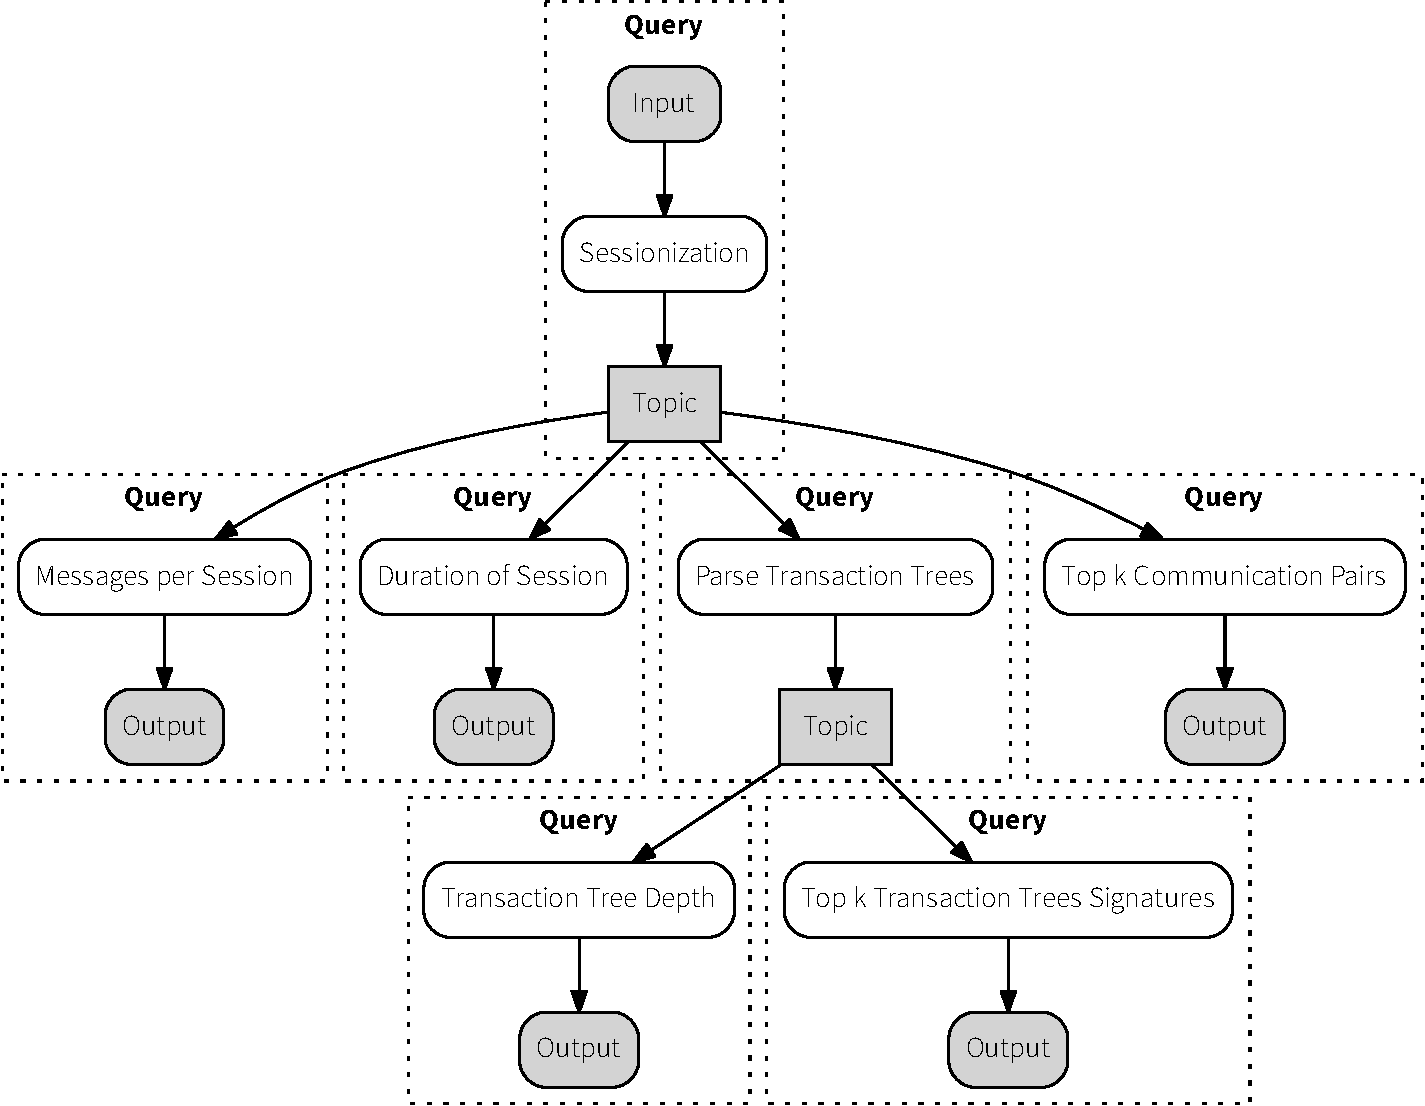
\includegraphics[width=1\textwidth]{figures/sessionize_split-crop}
  \caption[Dataflow graph for modular sessionization]{Structure of the modular
  sessionization. Two topics are introduced connect the tree of queries.}
  \label{fig:split}
\end{figure}

\paragraph{Topic Partitioning}

We maintain a simple one-to-one mapping between the number of topics and
number of worker threads in both the publishers and the subscribers.
Merging the stream partitions for publication and redistributing
the data at each subscriber would just result in unnecessary work.

\subsection{Worker-to-processor mapping}

We use the same amount of workers for each query to simplify topic partitioning.
But because the modular version naturally consists of more than one query,
the execution of the modular version will spawn more operating system threads
than the monolithic version.

For this reason we limit the the available CPU cores for the different executions,
ensuring the number of workers per query matches the number of available CPU cores.
Because our machine does have two processor sockets, each with their own memory bank,
the question arises how performance is impacted by different processor placement
policies. We explore this in section~\ref{sec:evalnuma}.

However, were not stated otherwise we prefer using as many physical cores 
as possible before falling back to hyper-threads, and we prefer filling the
first socket before allocating threads on the second socket. The memory
allocation policy is set up to always allocate on the local node.

Note that we do not pin individual worker threads to individual cores, we just
disallow access to excess cores. The operating system is free to load-balance
threads between the available cores.

\clearpage

\section{Results}

\subsection{Overhead in execution time}

We report the overall execution time of of both the monolithic and the 
modular query for different amounts of worker threads in Figure~\ref{fig:times}.

\begin{figure}[htb]
  \centering
    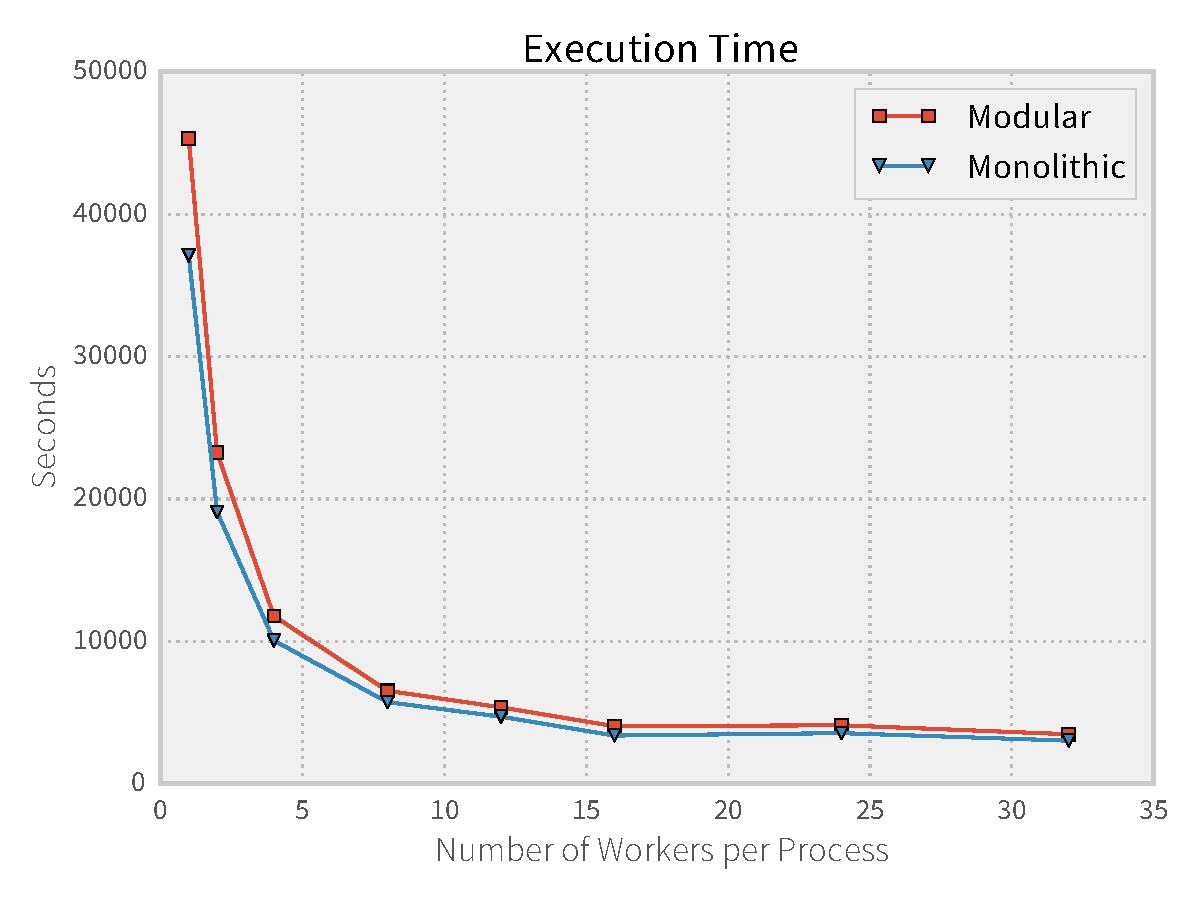
\includegraphics[width=1\textwidth]{figures/evaluation/times}

    {\footnotesize
    \vspace{1em}
    \begin{tabularx}{\textwidth}{ rXXXXXX }
      \hline 
      \textsc{Threads} & 4 & 8 & 12 & 16 & 24 & 32 \\
      \hline 
      \textsc{Overhead} & 17.2\%&13.7\%&14.0\%&18.8\%&14.4\%&13.5\% \\
      \hline
    \end{tabularx}
    }
    \caption[Execution times for different number of workers]{
    Execution times for different number of workers, for both the monolithic
    and the modular version.}
    \label{fig:times}
\end{figure}

As expected, we see that the modular version is slower than its monolithic
counterpart. Where the monolithic query uses in-memory queues to send data
to the next stage, the participants of modular version have to serialize
the messages and publish them in a topic. Both versions don't necessarily
perform better if we use hyper-threading for additional worker threads,
as 24 workers in both cases perform worse than 16.

The relative overhead varies between 13-18\%. Previous work has shown that
sessionization is able perform real-time processing on this machine with
16 workers and more. Our monolithic version is indeed also able to finish
the computation in under one hour with 16 workers and more. The modular version
however only achieves execution times below the threshold of one hour with
32 workers.

It should be noted that relative overhead is not proportional to the number
of worker threads. We will show in section~\ref{sec:evalnuma} that other
factors such as placement also impact the overhead.

\clearpage

\subsection{Worker utilization factor}

In this section we present the average measured utilization \emph{per worker},
i.e. the proportion of time a worker thread performs useful work.
This gives us an indicator of how well the different queries of the modular
version are able to cope with the given load.

We define the utilization factor of a worker as the percentage of
the time spent inside the Timely computation, i.e.
$\text{utilization} = \frac{\text{busy time}}{\text{total time}}$.
To put it another way, a worker is \emph{not busy} if it is waiting on external input.
This is the case if it wait on input from a topic in the case of the subscribers, 
or if it reads data from disk in the case of the sessionization stage.

Figure~\ref{fig:subutil} shows the average utilization for the subscribers, while
Figure~\ref{fig:sessutil} shows the utilization for the whole monolithic query
compared to the sessionization stage of the modular query. 

We see that in all cases the average utilization in the sessionization workers
is significantly higher than in the other queries of the modular version. This indicates
that the sessionization stage itself the bottleneck of the computation. 
We see that with a high number of worker threads, individual workers are proportionally
spending more and more time waiting for input.

This suggests that using the same amount of workers for all queries might
not be the most efficient use of computational resources. Future experiments would have to
explore how many worker threads are actually necessary for the different queries
in order to keep up. This however also requires a more sophisticated assignment of
topics to subscribing workers, which currently has to be manually encoded in
the queries source code.

\begin{figure}[p]
  \centering
    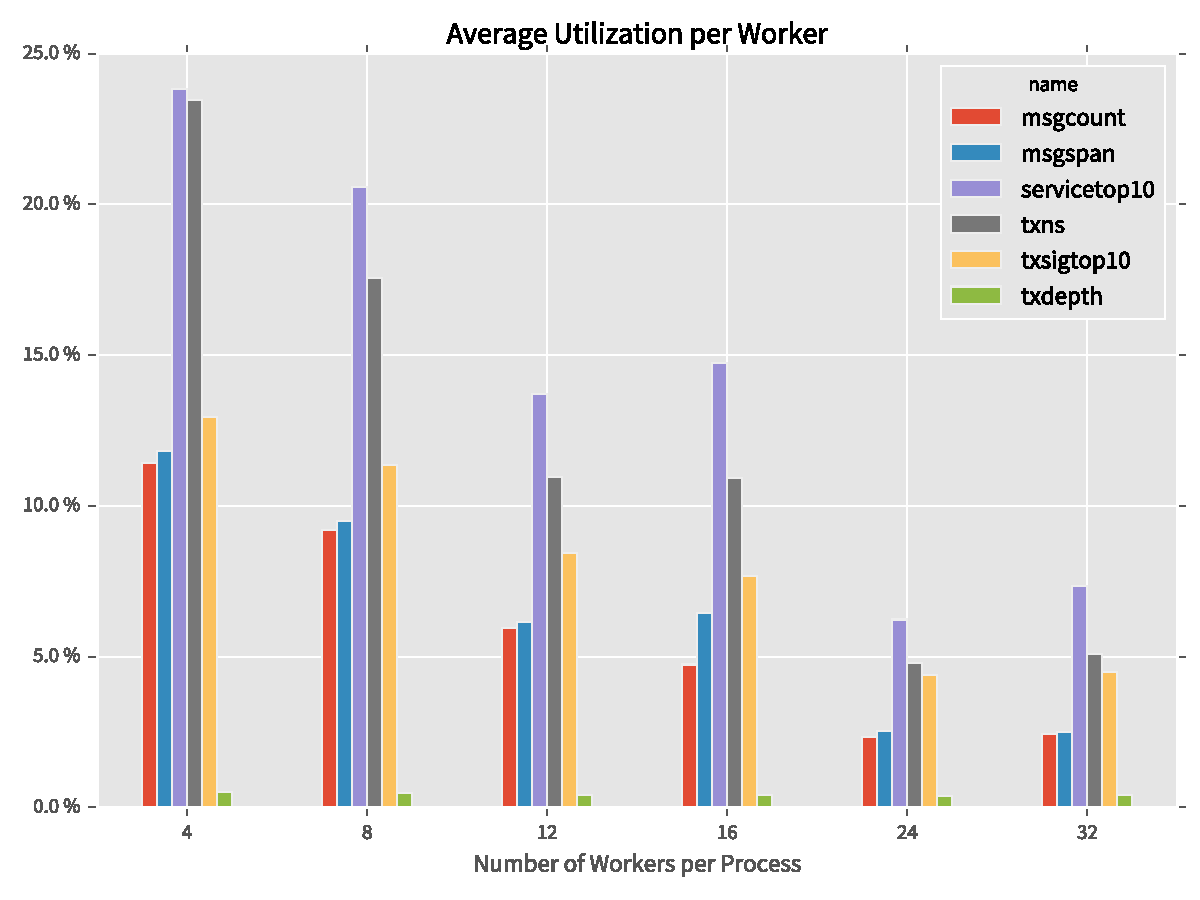
\includegraphics[width=1\textwidth]{figures/evaluation/subsutil}
    \caption[Subscriber worker utilization]{Utilization for the individual
    subscribers in the modular version.}
    \label{fig:subutil}
\end{figure}

\begin{figure}[p]
  \centering
    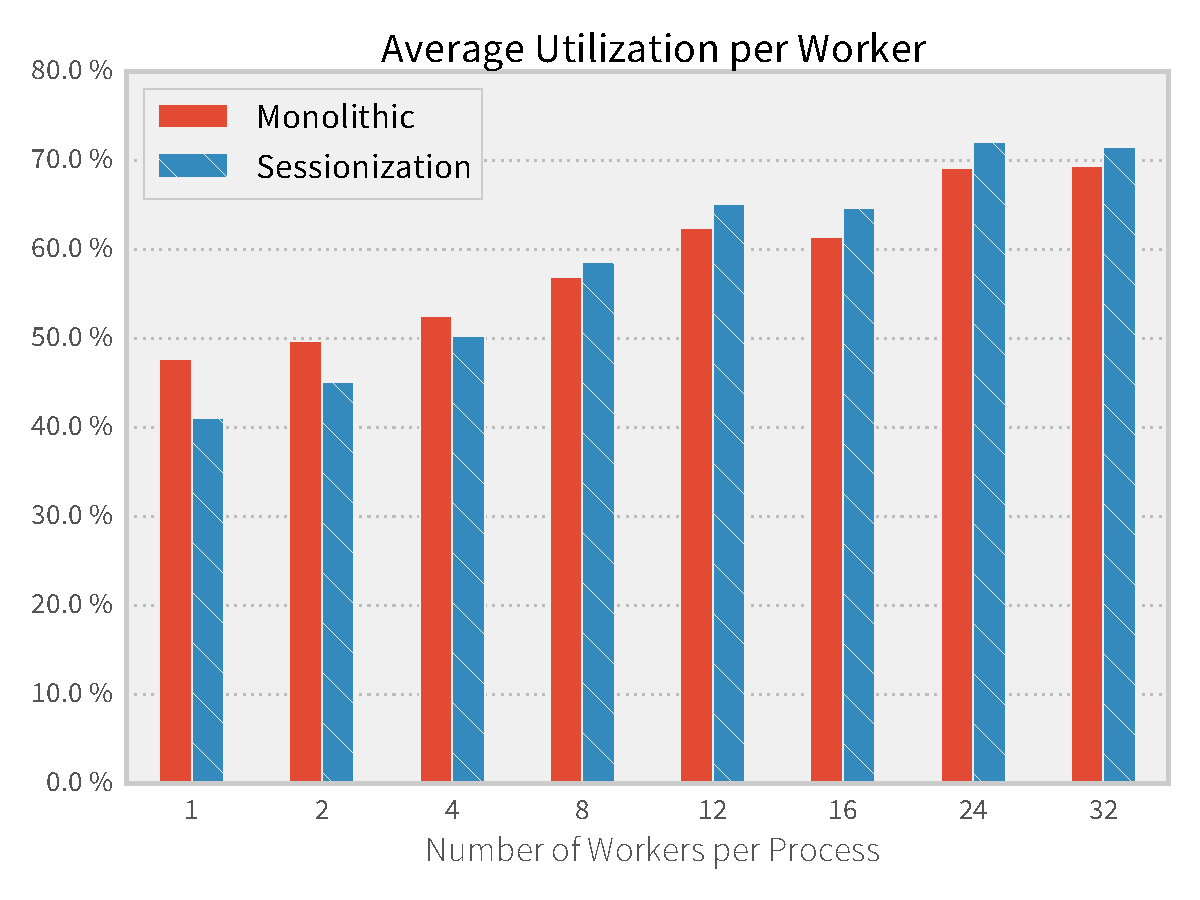
\includegraphics[width=1\textwidth]{figures/evaluation/sessutil}
    \caption[Sessionization worker utilization]{Utilization of the sessionization stage
    in the monolithic and the modular version.}
    \label{fig:sessutil}
\end{figure}
\clearpage
\subsection{Memory consumption and processor utilization}

Figures \ref{fig:rss} and \ref{fig:cpu} report the processor utilization and peak
memory consumption for the different processes, as reported by the operating
system.

\paragraph{Memory consumption}

We immediately see that the sessionization query of the composed version
consumes the most memory. This is caused by the fact that the re-ordering
and sessionization buffers incoming messages until certain epochs are completed.
Also with regard to the sessionization query, we see that its memory footprint
is higher than memory consumption for the monolithic version, even though
it performs less work. We assume that this is caused by the queuing of
outgoing messages at the publisher.

Another contributing factor to the overhead is the fact the we run additional
operating system processes, each one with a large set of worker threads.

\TODO{maybe split the figure in two separate figures, one for the subscribers
and one for sessionization}

\paragraph{Processor utilization}

We also report the overall processor utilization reported by the operating system.
A value of 100\% would correspond to the full utilization of all 32 logical cores.
We see that neither versions manage to fully utilize the processors over then duration of
the whole computation. This is indicates that both versions are sometimes blocked
on external input. Consistent with the observations from worker utilization, we
also see that the sessionization stage is the most compute heavy.

\begin{figure}[p]
  \centering
    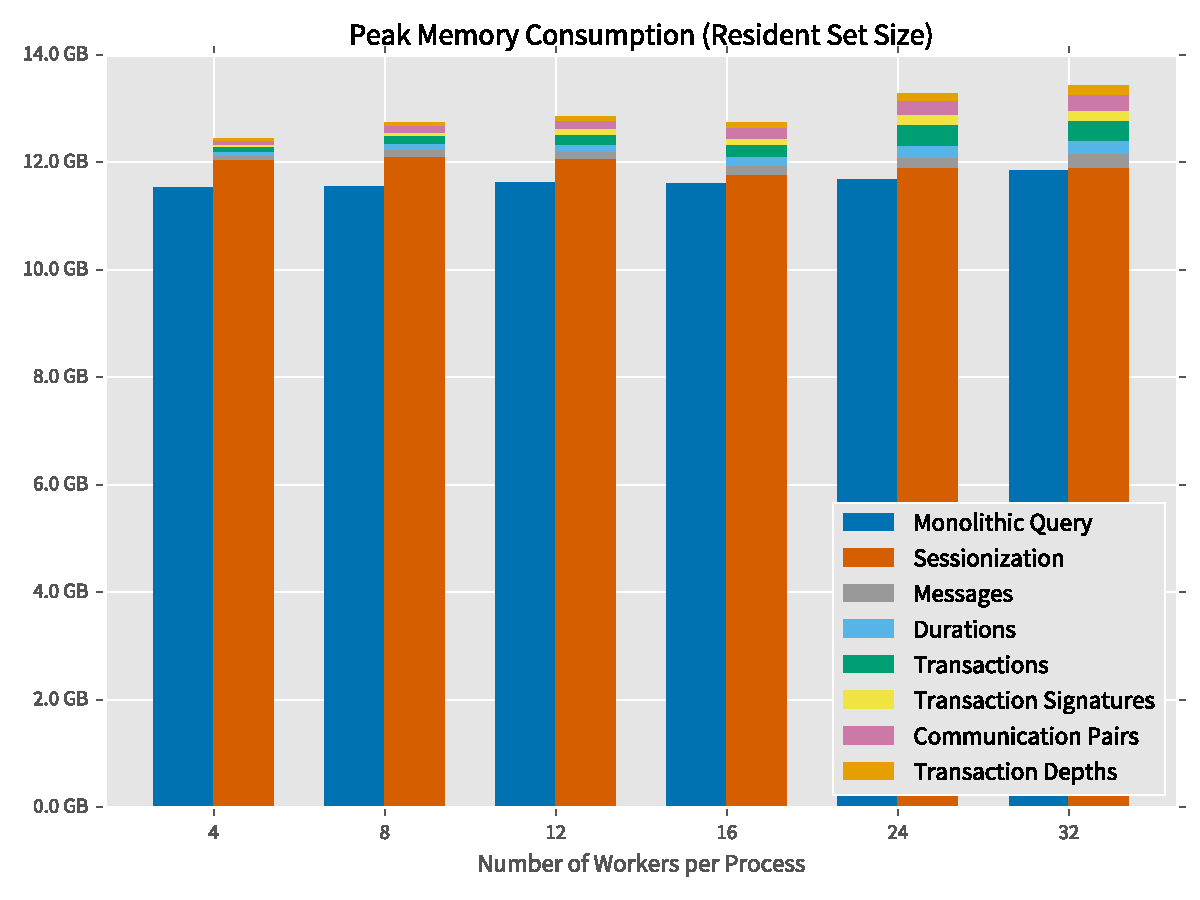
\includegraphics[width=1\textwidth]{figures/evaluation/rss}

    {\footnotesize
    \vspace{1em}
    \begin{tabularx}{\textwidth}{ rXXXXXX }
      \hline 
      \textsc{Threads} & 4 & 8 & 12 & 16 & 24 & 32 \\
      \hline 
      \textsc{Overhead} & 7.9\%&10.3\%&10.6\%&9.7\%&13.7\%&13.5\%\\
      \hline
    \end{tabularx}
    }
    \caption[Peak memory consumption]{Peak memory consumption of the different
    processes. The left bar shows the monolithic query, the right bar shows the memory
    used per query processed of the composed version.}
    \label{fig:rss}
\end{figure}

\begin{figure}[p]
  \centering
    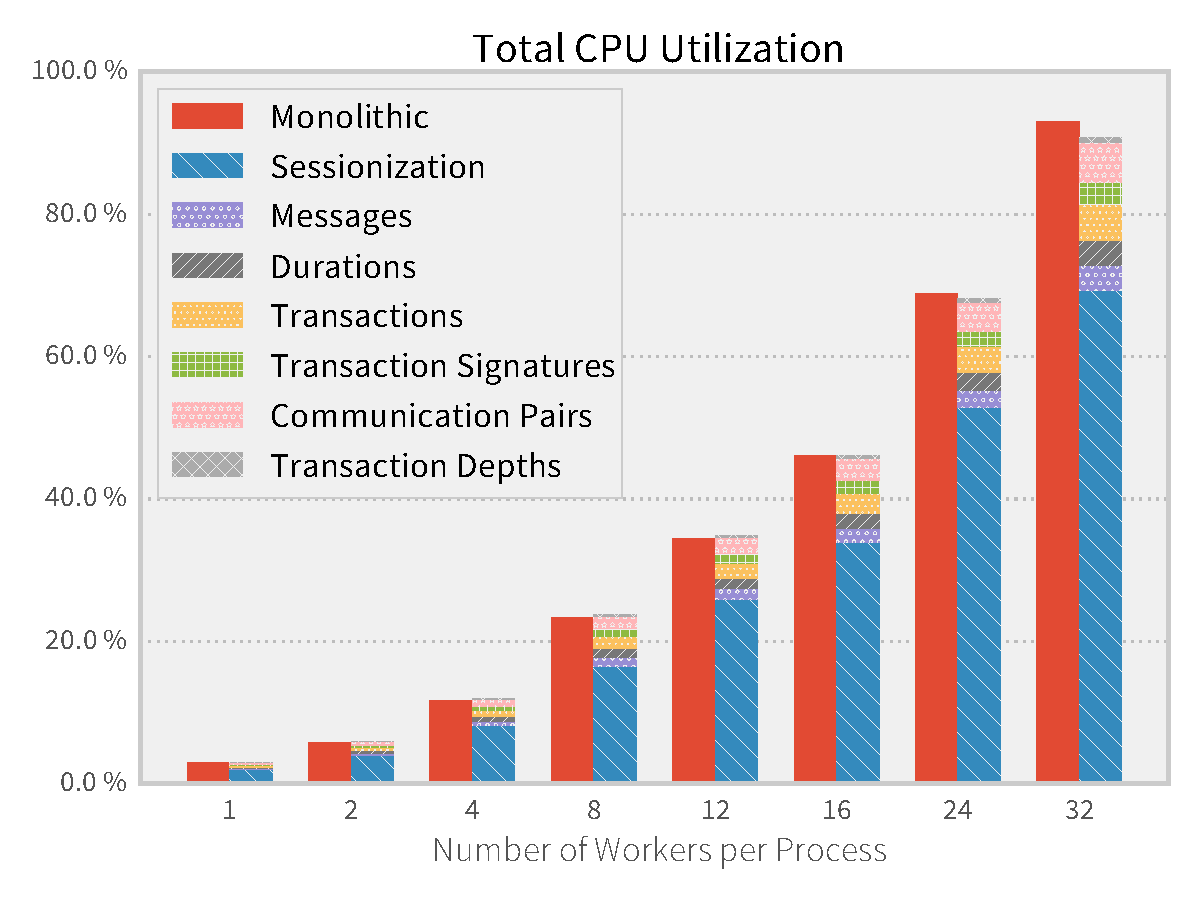
\includegraphics[width=1\textwidth]{figures/evaluation/cpu_tot}
    \caption[Total CPU utilization]{CPU utilization for the different
    processes. The left bar shows the monolithic query, the right bar shows the
    processor utilization for the different query processes in the modular version.}
    \label{fig:cpu}
\end{figure}
\clearpage
\subsection{Impact of worker placement} \label{sec:evalnuma}

In the above experiments, we prefer running as many workers as possible
on a single processor socket (with the exception of hyper-threads).
Figure~\ref{fig:numa} compares execution time of this strategy compared to a
strategy where we balance the workers evenly between sockets. With 12 workers
we are unable put all threads on a single socket, and we see that in this case
it is slightly beneficial to balance the threads evenly.

The impact of using different placements is relatively small for the
monolithic query. The modular version however is more sensitive to
different placement strategies, resulting in changes to the overhead
of the execution time. 

\begin{figure}[h]
  \centering
    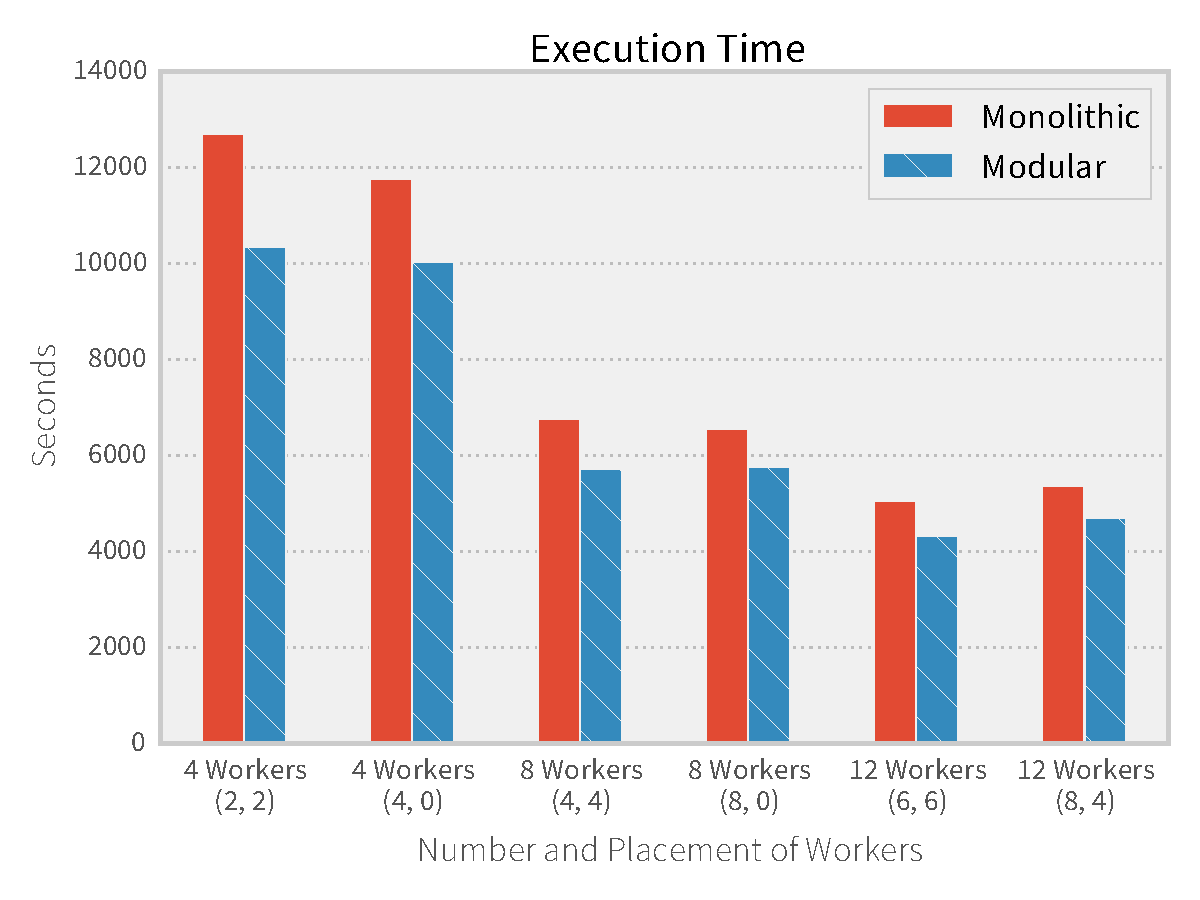
\includegraphics[width=1\textwidth]{figures/evaluation/numa}

    {\footnotesize
    \vspace{1em}
    \begin{tabularx}{\textwidth}{ r|XX|XX|XX }
      \hline 
      \textsc{Threads} & \multicolumn{2}{c|}{4} & \multicolumn{2}{c|}{8} & \multicolumn{2}{c}{12} \\
      \hline 
      \textsc{Placement} & (2, 2)&(4, 0)&(4, 4)&(8, 0)&(6, 6)&(8, 4)\\
      \hline 
      \textsc{Overhead} & 22.9\%&17.2\%&17.9\%&13.7\%&17.3\%&14.0\% \\
      \hline
    \end{tabularx}
    }
    \caption[Execution time for different of worker placement]{Execution times for
    different worker-to-processor mappings. The placement describes the number of
    worker threads placed on each of the two processor sockets.}
    \label{fig:numa}
\end{figure}

\clearpage
\subsection{Discussion}

In this chapter we presented an experimental evaluation of the overhead of
query composition in our system. The results show that the modular version in
our setting takes about 13-18\% longer to execute and consumes 8-14\% more
memory. While this is not negligible, we are confident that a modular version
of sessionization would be able to keep up with real-time processing, given
enough resources.

We believe though that further experiments are indispensable to definitely 
answer this question. Unfortunately we were not able to conduct more experiments
within the remaining time.

For one, future experiments should evaluate the performance of modular sessionization
in a cluster of machines. We only ran our experiments on a single machine, meaning that
data shared in topics was transmitted over the loopback interface.
Having publishers on one machine and subscribers on another would certainly yield
different performance characteristics. The monolithic version would also
likely show a different performance behavior, as workers would have to shuffle their data over the
network instead of using shared memory queues.

In addition, we did not perform any microbenchmarks to evaluate the performance
characteristics of other features of our system, such as the latency
of spawning a new query or the time it takes to subscribe to a topic. While
this would be interesting to evaluate, it currently would only be of little
significance for long-lived queries such as sessionization, as we expect
these features to be used mostly during the set-up phase of a query.
